\documentclass[12pt, twoside]{article}
\usepackage[letterpaper, margin=1in, headsep=0.5in]{geometry}
\usepackage[english]{babel}
\usepackage[utf8]{inputenc}
\usepackage{amsmath}
\usepackage{amsfonts}
\usepackage{amssymb}
\usepackage{tikz}
\usetikzlibrary{quotes, angles}
\usepackage{graphicx}
\usepackage{enumitem}
\usepackage{multicol}

\newif\ifmeta
\metatrue %print standards and topics tags

\title{Regents Geometry}
\author{Chris Huson}
\date{September 2020}

\usepackage{fancyhdr}
\pagestyle{fancy}
\fancyhf{}
\renewcommand{\headrulewidth}{0pt} % disable the underline of the header
\raggedbottom


\fancyhead[LE]{\thepage}
\fancyhead[RO]{\thepage \\ Name: \hspace{4cm} \,\\}
\fancyhead[L]{BECA / Dr. Huson / Geometry 05-Transformations\\* pset ID: 66}

\begin{document}

\subsubsection*{5-7DN-Segment-modeling}
\begin{enumerate}
\subsubsection*{Do Not Solve! \\
Label the drawing completely and write an equation in terms of $x$ modeling the situation.}
\vspace{0.5cm}

\item Given $\overline{ABC}$, with $AB=x-1$, $BC=3x+4$, and $AC=19$. Find ${AB}$. \vspace{1cm}
\begin{flushright}
  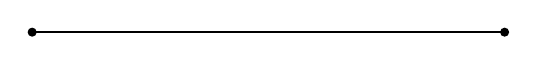
\begin{tikzpicture}
    \draw [-, thick] (0,0)--(6,0);
    \draw [fill] (0,0) circle [radius=0.05];
    \draw [fill] (6,0) circle [radius=0.05];
  \end{tikzpicture}
  \end{flushright} \vspace{2cm}

\item Given that $O$ bisects $\overline{NP}$. $NO=3x$, $OP=4x-7$. Find ${x}$. \vspace{1cm}
\begin{flushright}
  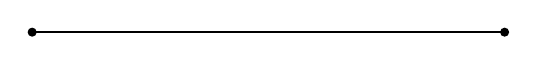
\begin{tikzpicture}
    \draw [-, thick] (0,0)--(6,0);
    \draw [fill] (0,0) circle [radius=0.05];
    \draw [fill] (6,0) circle [radius=0.05];
  \end{tikzpicture}
  \end{flushright} \vspace{2cm}
  
\item The points $R$, $S$, and $T$ are collinear, with $RS=3x-2$ and $ST=11$. If $RT=5x+1$, find ${RT}$. \vspace{1cm}
\begin{flushright}
  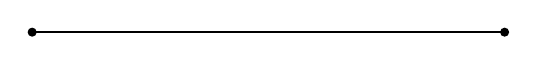
\begin{tikzpicture}
    \draw [-, thick] (0,0)--(6,0);
    \draw [fill] (0,0) circle [radius=0.05];
    \draw [fill] (6,0) circle [radius=0.05];
  \end{tikzpicture}
  \end{flushright} \vspace{2cm}
  
\item The point $K$ is the midpoint of $\overline{JL}$, $JK=3x+8$, and $JL=8x+36$. Find ${JK}$.  \vspace{1cm}
\begin{flushright}
  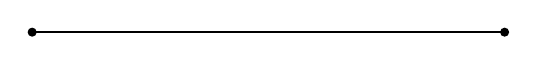
\begin{tikzpicture}
    \draw [-, thick] (0,0)--(6,0);
    \draw [fill] (0,0) circle [radius=0.05];
    \draw [fill] (6,0) circle [radius=0.05];
  \end{tikzpicture}
  \end{flushright} \vspace{2cm}

\end{enumerate}
\end{document}